\chapter{The DSNB NCQE background}
\epigraph{``Mr. Scott cannot give me exact figures, Admiral, so... I will make a guess.''}{Mr. Spock, Star Trek IV: The Voyage Home (1986)}
\label{chp:ncqe_xsec}


\section{Introduction}

As mentioned in Chapter 1, NCQE interactions form the main background to the DSNB signal, and therefore calculating the number of events that form this background concludes the work of this analysis. 

The number of observed neutrino events which are detected at Super-Kamiokande as a function of some observable such as reconstructed neutrino energy $N_{\nu}(E_{\nu})$ is given in Equation \ref{eq:nu_number}.

\begin{equation}
    N_\nu(E_\nu)=\mathcal{C} \int \Phi\left(E_\nu\right) \sigma\left(E_\nu\right) \epsilon d E_\nu
\label{eq:nu_number}
\end{equation}

Here, $\mathcal{C}$ is the target volume, $E_{\nu}$ is the true incoming neutrino energy, $\Phi(E_{\nu})$ is the flux of the incoming neutrino, $\sigma(E_{\nu})$ is the cross section for the neutrino interaction and $\epsilon$ is the detection efficiency of the neutrino by the far detector. The number of neutrino events from Monte Carlo for each interaction type is given by summing the number of NCQE events for neutrinos and anti-neutrinos, and charged-current and NC-other interactions, where the numbers of the neutrino and antineutrino NCQE events are multiplied by scale factors which scale the simulated NCQE cross section prediction.




\section{NCQE cross-section uncertainty prediction}


The number of events $N_{obs}$ are made up of the sum of the signal ($S$) and background ($B$) events, i.e: $N_{obs} = S + B$. The signal events are described by the summation of the number of neutrino and antineutrino NCQE events multiplied by their scale factors: $S  = f_{\nu-\mathrm{NCQE}} M_{\nu-\mathrm{NCQE}}^{\mathrm{FHC}}+f_{\bar{\nu}-\mathrm{NCQE}} M_{\bar{\nu}-\mathrm{NCQE}}^{\mathrm{FHC}}$ for FHC mode. These scale factors are used to scale the NCQE cross section predictions made by NEUT. By having a similar equation for RHC mode, one can produce the Equations in \ref{eq:scale_factor_nu}, where $X$ and $Y$ are the number of background events for FHC and RHC mode respectively, which give the scale factor values for neutrino and antineutrino NCQE interactions. 

\begin{equation}
    \begin{aligned}
    f_{\nu-\mathrm{NCQE}}= & \frac{X M_{\bar{\nu} \mathrm{N} \mathrm{NCQE}}^{\mathrm{RHC}}-Y M_{\bar{\nu}-\mathrm{NCQE}}^{\mathrm{FHC}}}{M_{\nu-\mathrm{NCQE}}^{\mathrm{FHC}} M_{\bar{\nu}-\mathrm{NCQE}}^{\mathrm{RHC}}-M_{\nu-\mathrm{NCQE}}^{\mathrm{RHC}} M_{\bar{\nu}-\mathrm{NCQE}}^{\mathrm{FHC}}} \\
    f_{\bar{\nu}-\mathrm{NCQE}}= & \frac{X M_{\nu-\mathrm{NCQE}}^{\mathrm{RHC}}-Y M_{\nu-\mathrm{NCQE}}^{\mathrm{FHC}}}{M_{\bar{\nu}-\mathrm{NCQE}}^{\mathrm{FHC}} M_{\nu-\mathrm{NCQE}}^{\mathrm{RHC}}-M_{\bar{\nu}-\mathrm{NCQE}}^{\mathrm{RHC}} M_{\nu-\mathrm{NCQE}}^{\mathrm{FHC}}}
    \end{aligned}
\label{eq:scale_factor_nu}
\end{equation}


Table \ref{table:nu_FHC_mc} gives the expected number of neutrino events for each type of interaction including neutral current and charged current interactions for FHC mode for a predicted future POT of $10 \times 10^{21}$ by Japanese Fiscal Year 2028 \cite{Abe:2016tii}, and Table \ref{table:nu_RHC_mc} shows the same information for RHC mode. These have been calculated with the 21bv2 flux uncertainty tuning. Figure \ref{fig:erec_fhc_rhc_2728} shows the number of events plotted against the reconstructed energy ($E_{rec}$) of the event for FHC and RHC mode.

\begin{figure}
    \centering
    
    \begin{minipage}{0.49\textwidth}
        \centering
        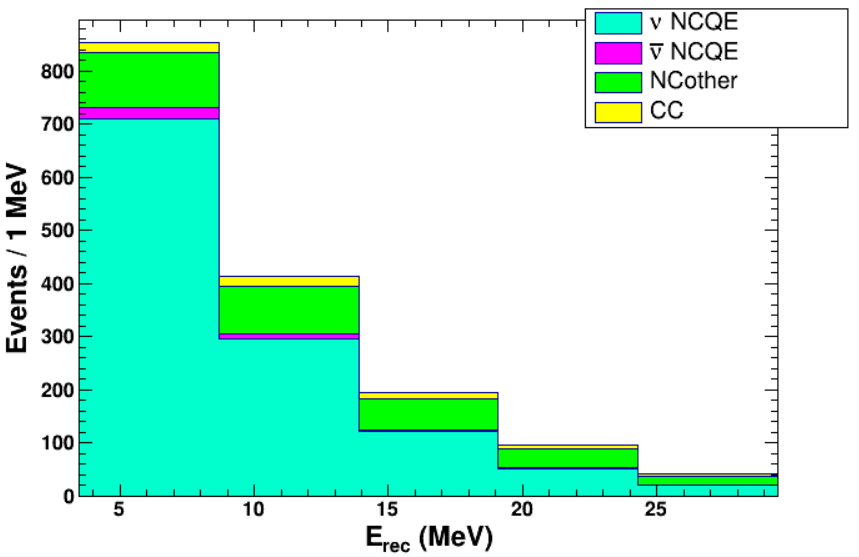
\includegraphics[width=\textwidth]{Figures/erec_2728_POT_FHC.PNG} % first figure itself
        \caption{Number of events plotted against $E_{rec}$ for T2K FHC mode }
    \end{minipage}\hfill
    \begin{minipage}{0.49\textwidth}
        \centering
        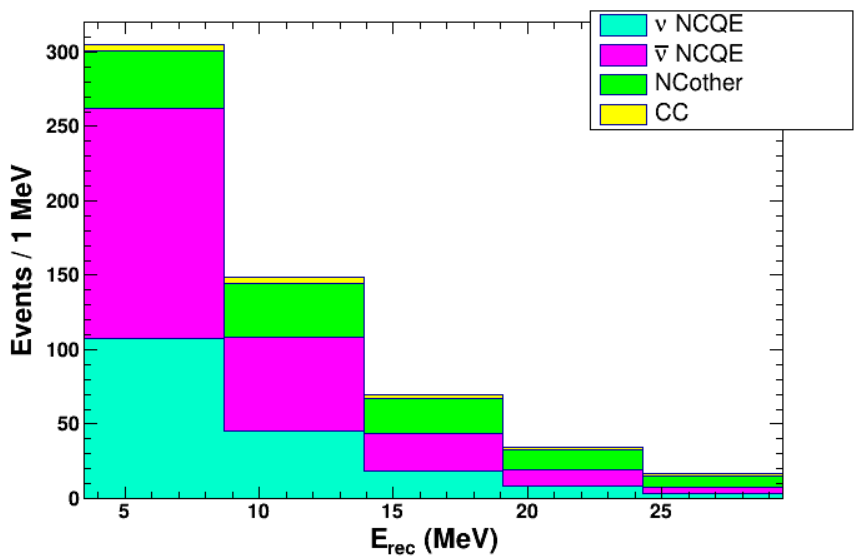
\includegraphics[width=\textwidth]{Figures/erec_2728_POT_RHC.PNG} % second figure itself
        \caption{Number of events plotted against $E_{rec}$ for T2K RHC mode}
        \label{fig:erec_fhc_rhc_2728}
    \end{minipage}
\end{figure}


\begin{table}
    \centering
    \begin{tabular}{||ccc||}
        \hline FHC sample & MC $\# \nu_{\mathrm{det}}$ & MC $\# \nu_{\mathrm{det}}$ fraction $(\%)$ \\
        \hline$\nu-N C Q E$ & 1199.7 & 75.0 \\
        $\bar{\nu}-\mathrm{NCQE}$ & 34.5 & 2.2 \\
        $N C-$ other & 288.1 & 19.1 \\
        $C C$ & 17.4 & 3.7 \\
        \hline Total & 1599.2 & 100 \\
        \hline
        \end{tabular}        
    \caption{FHC MC expectation values for each interaction type with a total SK POT of $10 \times 10^{21}$}
    \label{table:nu_FHC_mc}
\end{table}


\begin{table}
    \centering
    \begin{tabular}{||ccc||}
        \hline RHC sample & MC $\# \nu_{\text {det }}$ & MC \# $\nu_{\text {det }}$ fraction $(\%)$ \\
        \hline$\nu-N C Q E$ & 182.8 & 31.9 \\
        $\bar{\nu}-$ NCQE & 257.0 & 44.8 \\
        $N C-$ other & 118.4 & 20.6 \\
        $C C$ & 15.3 & 2.7 \\
        \hline Total & 573.5 & 100 \\
        \hline
    \end{tabular}
    \caption{RHC MC expectation values for each interaction type with a total SK POT of $10 \times 10^{21}$.}
    \label{table:nu_RHC_mc}
\end{table}

Due to this being a future prediction of the background rate using MC and not data, $N_{obs}$ is the total number of events in the MC, meaning that the value of the scale factor is 1.00. However, the uncertainty on the scale factor is not trivial, and Equation \ref{eq:scale_factor_uncertainty} shows how it is calculated.

\begin{equation}
    \delta_{f} = \left({\frac{\sqrt{N_{\text{obs}}}}{N_{\text{obs}}}}\right)^{2} + \left({\frac{\delta_{\epsilon}}{\epsilon}}\right)^{2}
\label{eq:scale_factor_uncertainty}
\end{equation}

The values for the uncertainty on the scale factors for FHC and RHC mode is shown in Equation \ref{eq:scale_factors}.


\begin{equation}
    \begin{aligned}
    & \delta{f_{\nu-\mathrm{NCQE}}}= \pm 0.129 \\
    & \delta{f_{\bar{\nu}-\mathrm{NCQE}}}= \pm 0.133
    \label{eq:scale_factors}
    \end{aligned}
\end{equation}


\section{Number of DSNB NCQE background events}

The number of DSNB NCQE background events is given by Equation \ref{eq:background_events}. 

\begin{equation}
N_{B} = \mathcal{C} \epsilon_{N} f\int \Phi(ATM) \epsilon_{N} \sigma(E_{\nu}) d E_{\nu} 
\label{eq:background_events}
\end{equation}

Where $\mathcal{C}$ is the target volume, $\Phi(ATM)$ is the atmospheric neutrino flux, $\sigma$ is the neutrino interaction cross section, $\epsilon_{N}$ is the neutron tagging efficiency and $f$ is the value of the scale factors. In 2021 the Super-Kamiokande DSNB analysis working group released the first results showing the number of low energy inverse beta decay events in MC and data for 552.2 days of SK-Gd data. Table \ref{table:DSNB_analysis} shows the number of events for MC and data for each energy bin of 2 MeV in the 8-30 MeV signal region. Figure \ref{fig:DSNB_hist} shows the energy spectrum of these events in the signal region after data reduction and neutron tagging, along with the associated backgrounds.

\begin{table}[!htb]
\centering
\begin{tabular}{||ccc||}
\hline
$\text{ Energy (MeV)}$ & $\text{ Obs. (/bin) }$ & $\text{ Exp. (/bin) }$\\
\hline 
8-10 & 7 & 9.18 $\pm$ 3.58 \\
10-12 & 4 & 2.78 $\pm$ 0.93 \\
12-16 & 0 & 1.05 $\pm$ 0.21 \\
16-24 & 2 & 0.41 $\pm$ 0.09 \\
24-30 & 1 & 0.41 $\pm$ 0.07 \\
\hline
\end{tabular}
\caption{Number of low energy IBD events for each 2 MeV energy bin from 8 - 30 MeV for data and MC}
\label{table:DSNB_analysis}
\end{table}


\begin{figure}[!htb]
    \centering
    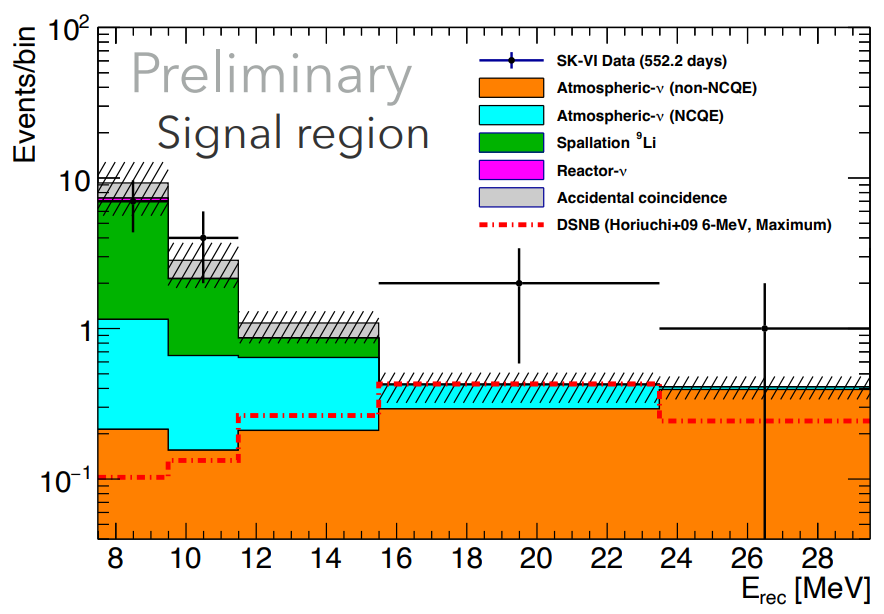
\includegraphics[width=0.8\textwidth]{Figures/DSNB_hist.png}
    \caption{Reconstructed energy spectra after data reduction for the backgrounds and the observed data taken with 552.2 days of SK-VI data. Taken from \cite{DSNBhist}, accessed on 22/03/23.}
    \label{fig:DSNB_hist}
\end{figure}

Scaling the total number of events found from the MC in Figure \ref{fig:DSNB_hist}, (2.04 events) from the 552.2 days of taking data to 2028 gives 9.88 events in FHC mode. Using Equation \ref{eq:background_events}, the number of predicted DSNB NCQE background events for FHC mode is given in Equation \ref{eq:DSNB_NCQE}, with the combined systematic and statistical error on this value calculated as in Equation \ref{eq:DSNB_NCQE_error}.

\begin{equation}
    \left(\frac{\delta_{N_{\nu-\mathrm{DSNB}_{NCQE}}}}{N_{\nu-\mathrm{DSNB}_{NCQE}}}\right)^{2} = \left({\frac{\sqrt{N_{\text{obs}}}}{N_{\text{obs}}}}\right)^{2} + \left({\frac{\delta_{\epsilon_{N}}}{\epsilon_{N}}}\right)^{2} + \left({\frac{\delta_{f}}{f}}\right)^{2}
\label{eq:DSNB_NCQE_error}
\end{equation}


\begin{equation}
    \begin{aligned}
        & N_{\nu-\mathrm{DSNB}_{NCQE}}= 9.88 \pm 3.62 \\
    \label{eq:DSNB_NCQE}
    \end{aligned}
\end{equation}

To summarise, as shown in Figure \ref{fig:DSNB_hist}, the dominant atmospheric neutrino background comes from NCQE interactions, and cross section measurements from T2K can be used to estimate this background. Monte Carlo simulations of neutrino and anti-neutrino NCQE interactions can be renormalised using scaling factors from data, while the error on these scale factors are taken as cross-section uncertainties. Values of these scale-factor errors are given in Equation \ref{eq:scale_factors} and these have been calculated from the expected number of neutrino events for a future POT of $10 \times 10^{21}$ starting JFY 2028, shown in Table \ref{table:nu_FHC_mc} and Table \ref{table:nu_RHC_mc}. The number of DSNB NCQE background events in MC are taken from results from SK-Gd in 2021 and scaled up to the JFY 2028 prediction, with the error on the scale factor used to produce the total uncertainty (Equation \ref{eq:DSNB_NCQE_error}) on this measurement. The estimation of DSNB NCQE background error is important because of NCQE interactions being the dominant atmospheric neutrino background below 15 MeV and its the constraining of this background which is fundamental to DSNB searches. 

